\subsection{Implementation of Methods for Data Collection and Data Analysis}

This section describes the implementation of methods for each iteration's interactions, in regards to collecting and analysing qualitative and quantitative data. Figure \ref{fig:methods} is made to assist the reader in the iterations' different focuses.

%study design, application development, and for data analysis theory.

\begin{figure}[h]
    \centering
    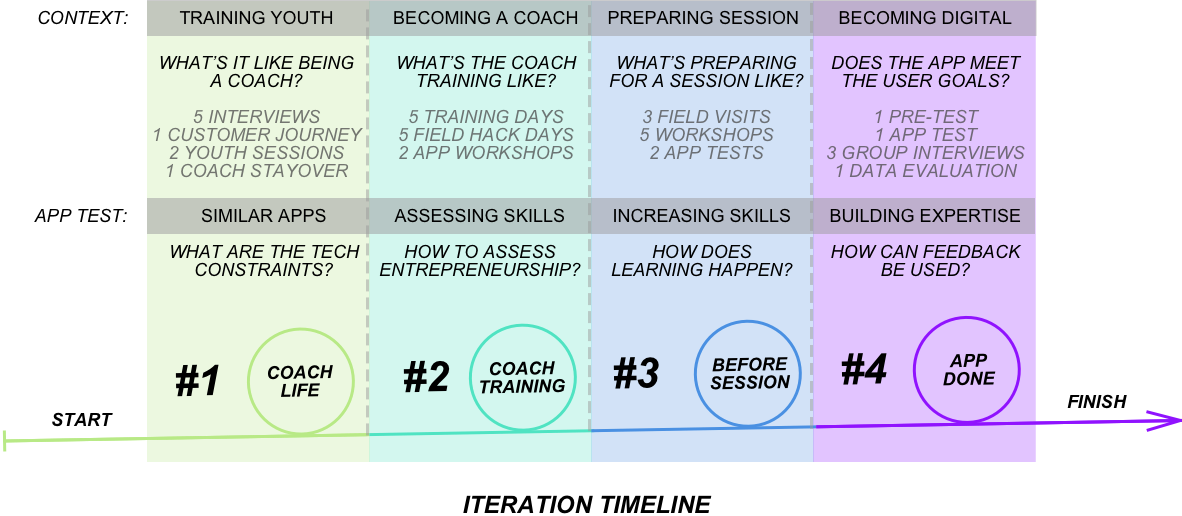
\includegraphics[width=1.0\textwidth]{iterativeprocess2.png}
    \caption{Each of the four iterations had a unique context, app test focus, and research focus. The loops is meant to remind that an iteration consists of three steps before Interactions with the coaches: Insights, Ideation and Trigger material. For more information, see section \ref{digital-service-design} Digital Service Design.}
    \label{fig:methods}
\end{figure}

%Methods w/ Analysis
%----
%
%5 Interviews - Notes - Questionnaire for Customer Journey
%1 Customer Journey - Clustering - Personas
%2 Youth Sessions - Shadowing - Needs
%1 Coach Stayover - Empathy - Design Ethnography
%
%5 Training Days - Observations - Understanding entrepreneurship training
%5 Hackathon Days - Interviews - Notes and Sketches
%2 App Workshops - Co-Creation/Co-Refinement - Sketches and Needs
%
%3 Field
%
%Acitivity
%App test observations (group)
%
%App test observation (individual)
%- Affective reactions (5 Why's, think aloud)
%
%Analysis: Interaction design evaluation (desirability, usability, utility, %pleasurability)
%
%Customer Journey Map
%- Activities
%- Behaviour
%
%Written responses (individual)
%- Right/wrong
%- Time
%- Number of tries
%
%Interviews
%- New insights
%
%Data Collection w/ Analysis
%----
%
%Customer Journey Map w/ clustering
%
%Pre-study w/ Quantative analysis
%
%Written quiz responses w/ Quantative analysis
%
%Digital quiz responses / Quantative analysis + Statistical analysis + %Parallell coordinates
%
%Quiz questions 1 w/ Bloom analysis
%Quiz questions 2 w/ Bloom analysis

%\input{implementation/iteration-1}

%\input{implementation/iteration-2}

%\input{implementation/iteration-3}

%\input{implementation/iteration-4}
